\documentclass[12pt,letterpaper]{article}
%\usepackage{fullpage}
\usepackage[top=2cm, bottom=4.5cm, left=2.5cm, right=2.5cm]{geometry}
\usepackage{amsmath,amsthm,amsfonts,amssymb,amscd}
%\usepackage{lastpage}
\usepackage{enumerate}
\usepackage{fancyhdr}
%\usepackage{mathrsfs}
\usepackage{xcolor}
\usepackage{graphicx}
\usepackage{listings}
\usepackage{hyperref}
\usepackage{tikz}

\hypersetup{%
  colorlinks=true,
  linkcolor=blue,
  linkbordercolor={0 0 1}
}
 
\renewcommand\lstlistingname{Algorithm}
\renewcommand\lstlistlistingname{Algorithms}
\def\lstlistingautorefname{Alg.}

\lstdefinestyle{Python}{
    language        = Python,
    frame           = lines, 
    basicstyle      = \footnotesize,
    keywordstyle    = \color{blue},
    stringstyle     = \color{green},
    commentstyle    = \color{red}\ttfamily
}

\setlength{\parindent}{0.0in}
\setlength{\parskip}{0.05in}

% Edit these as appropriate

\pagestyle{fancyplain}
\headheight 35pt
\lhead{DS 211 \\ Numerical Optimization}                 % <-- Comment this line out for problem sets (make sure you are person #1)
\chead{\textbf{\Large Lecture 17}}
\rhead{Scribe: Shriram R.}
\lfoot{}
\cfoot{}
\rfoot{\small\thepage}
\headsep 1.5em

\newcommand{\R}{\mathbb{R}}


\begin{document}

\section{Standard Form}

The standard form of a linear programming problem is as follows,

\begin{equation*}
\min c^{T}x, \text{ subject to } Ax = b, x \geq 0,
\end{equation*}

where $A \in \R^{m \times n}$, $c$ and $x$ $\in \R^{n\times1}$ and $b \in \R^{m\times1}$. Also, $m \leq n$ and Rank$(A) = m$. Often, framing a linear programming problem in the standard form is an important task itself.

\section{Revised Simplex Algorithm}

\begin{figure}[h]
	\centering
	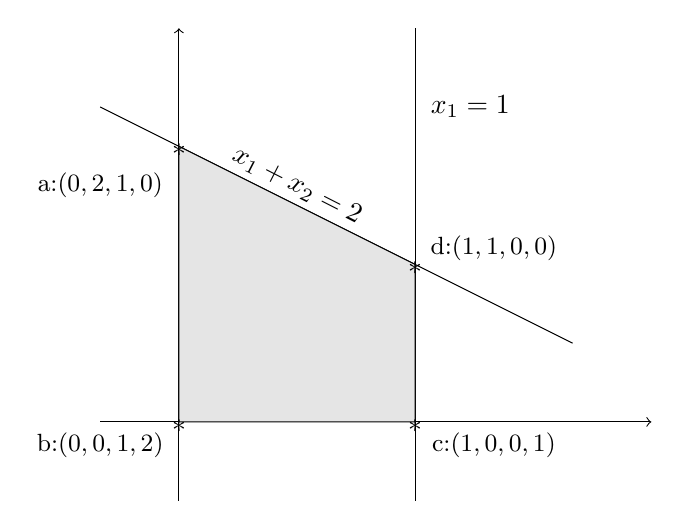
\begin{tikzpicture}
	\draw [->] (5,-1) -- (5,5);
    \draw [->] (4,0) -- (11,0);
	\draw [] (4,4) -- (10,1);
	\draw [] (8,-1) -- (8,5);
	\filldraw[draw=black, fill=gray!20] (5,0) -- (8,0) -- (8,2) -- (5,3.5) -- cycle;
	\node[] at (8.7,4) {$x_1 = 1$};
	\node[rotate=-27] at (6.5,3) {$x_1 + x_2 = 2$};
	\node[] at (8,-0.1) {*};
	\node[] at (8, 1.9) {*};
	\node[] at (5, -0.1) {*};
	\node[] at (5, 3.4) {*};
	\node[] at (4,3) {\small{a:$(0,2,1,0)$}};
	\node[] at (4,-0.3) {\small{b:$(0,0,1,2)$}};
	\node[] at (9,-0.3) {\small{c:$(1,0,0,1)$}};
	\node[] at (9,2.2) {\small{d:$(1,1,0,0)$}};
	\end{tikzpicture}
	\caption{Constraints and vertices of the polytope}
	\label{fig1}
\end{figure}

Let us consider the following linear programming problem as an example, 
\begin{equation*}
\min \text{ } x_1+2x_2, \text{ subject to } x_1 \leq 1 \text{, } x_1 + x_2 \leq 2\text{, } x_1 \geq 0\text{, } x_2 \geq 0
\end{equation*}
Adding slack variables $x_3$ and $x_4 \in S$ to the constraints to convert to standard form, we get,
\[
A =  \begin{bmatrix}
1 & 0 & 1 & 0 \\
1 & 1 & 0 & 1
\end{bmatrix}
, b = \begin{bmatrix}
1 \\
2
\end{bmatrix}
, c = \begin{bmatrix}
1 \\
2
\end{bmatrix}
\]

Figure:~\ref{fig1} illustrates the constraints and the four vertices of the feasible polytope formed by the constraints of the above example. It can be observed that exactly 2 out of 4 variables are non-zero (active) since Rank$(A)=2$ and exactly 1 variable changes to active and 1 variable changes to inactive when we move one vertex to any of its neighbouring vertices.

Also, the solution to this problem lies in one of the vertices of the feasible polytope. This means we have to iterate over $n_{C_m}$ possible vertices to find the optimum solution in a brute force approach. This is combinatorially expensive and so simplex method provides an efficient way of searching this set of vertices.

\subsection{Definitions}

\begin{itemize}
	\item $\mathcal{B}$ denotes the subset of index set $\mathcal{I} = \{1,2,\dots,n\}$ containing exactly $m$ indices such that $i \notin \mathcal{B} \implies x_i = 0$. This is called the basic set.
	\item $B = [A_i]_{i \in \mathcal{B}}$ denotes a non-singular $m\times m$ matrix called as the basic matrix.
	\item $\mathcal{N}$ denotes the non-basic set $\mathcal{N} = \{1,2,\dots,n\}\setminus\mathcal{B}$ containing $n-m$ indices such that $i \in \mathcal{N} \implies x_i = 0$.
	\item $N = [A_i]_{i \in \mathcal{N}}$ denotes a $m\times (n-m)$ matrix called as the non-basic matrix.
	\item $x, c \text{ and } S$ are partitioned as basic and non-basic vectors and are defined as below,
	      \begin{center}
				$x_B = [x_i]_{i \in \mathcal{B}}$ ~~~~~~ $x_N = [x_i]_{i \in \mathcal{N}}$ \\
				$c_B = [c_i]_{i \in \mathcal{B}}$ ~~~~~~ $c_N = [c_i]_{i \in \mathcal{N}}$ \\
				$S_B = [S_i]_{i \in \mathcal{B}}$ ~~~~~~ $S_N = [S_i]_{i \in \mathcal{N}}$ \\
	      \end{center}		  
\end{itemize}

\subsection{Algorithm}

\end{document}